\section{Dataset}

We ran multiple iterations of the recording process to find the best possible setup, which reduces the light interference as much as possible and which offers the best results with the resources at hand. We reproduced the setup of the camera as it is used at SilverFit. At SilverFit the camera is mounted at $175cm$. The camera is angled downward at a $70^\circ$ angle. We measure the height with a measuring tape. To estimate the correct angle is very difficult. Thankfully, the Realsense Camera provides us with an accelerometer, which measures the acceleration of the camera. Therefore, it also measures the gravity. An example of the measurements can be seen in Figure \ref{fig:accellerometer}. With these measurements we can calculate the percentage of downward force and know the exact angle at which the camera is to the ground. Additionally, we can fix any roll of the camera providing us with a straight image. 

\begin{equation} \label{eq:orientation}
\dfrac{y}{x+y+z} * 90^{\circ} = Angle
\end{equation}

Equation \ref{eq:orientation} was used to achieve the specified orientation. In our case the target angle in degree is $70^\circ$. Therefore, we know that ${y}/{(x+y+z)} * 90^{\circ} = 70^{\circ}$. Since we eliminated the roll prior we know that $x=0$. Hence, we know that to achieve an angle of 70 degrees, ${y}/{(y+z)}$ has to be equal to ${70^\circ}/{90^\circ}$. The values of $z$ and $y$ can be seen in Figure \ref{fig:accellerometer}. In the Figure $z \approx -3.923 {m}/{s^2}$ and $y \approx -8.855 {m}/{s^2}$, therefore, ${y}/{(y+z)} * 90^\circ = 62.3 \neq 70$ so the camera needs to be rotated further. This process has to be repeated until the angle is correct.

\begin{figure}
  \centering
  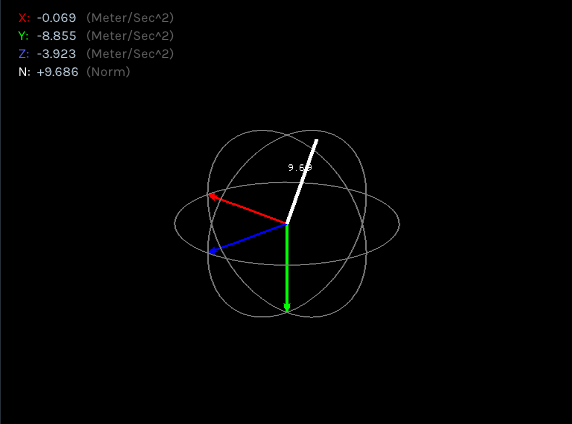
\includegraphics[width=0.5\textwidth]{figures/FESD/accelerometer.png}
  \caption[Realsense Accelerometer]{Accelerometer data from the Realsense camera used to set up the camera.}
  \label{fig:accellerometer}
\end{figure}

\subsection{Analysis}

An important aspect of the dataset is the structure and distribution of data and their labels. In total we recorded all 13 exercises, mentioned in Section \ref{sec:exercises}, twice. Each recording session consists of exactly 300 frames.

If a joint cannot be detected by Nuitrack it automatically gets zero coordinates, i.e. every value is zero. This makes it easy to automatically label these joints as faulty, in particular with the error label $1$ - Joint Missing. However, for the rest of the errors each frame has to be manually inspected and each joint considered. Since this requires a lot of work we reduced the labeled frames to 10 percent of the original size. Therefore, each exercise contains 30 frames and in total $30 \cdot 13 \cdot 2 = 720$ frames are labeled.

When multiple persons are detected one person might be incorrectly detected in the background. While analysing the data we pick the person that is not labeled as faulty whenever possible. For training and testing this is choosen at random. If a person is labeled as faulty each joint is marked as in a unrealistic position.

\subsubsection{Distribution of Errors}

An important factor in how well a model can be trained on data is the balance of the dataset. In this case, the dataset is balanced by the error labels. In Figure \ref{fig:statistics_err_dist} we can see the distribution of errors in the dataset as a whole. We see that most of the joints are not faulty, i.e. are in the position they are supposed be within a margin of error.

\begin{figure}
  \centering
  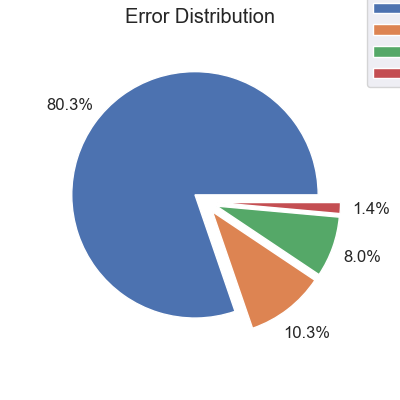
\includegraphics[width=0.5\textwidth]{figures/Data/Error_Distribution.png}
  \caption[Error Distribution]{The distribution of errors TODO}
  \label{fig:statistics_err_dist}
\end{figure}

To diversify the dataset we recorded different exercises with varying difficulties. In Figure \ref{fig:statistics_err_diff} we see that the difficulty has an influence on the amount of errors that occur for any given joint. We see that there is barely any difference between the trivial and the easy exercises. However, in Figure \ref{fig:statistics_err_dist_diff} we see that while trivial exercises have a higher percentage of unrealistic joint positions, i.e. the joint is in a wrong location, the easy exercises have a higher percentage of joints which are not detected. However, this difference is very small. Medium and Hard exercises are more error prone as was intended. This reflects our design proposals for challenging exercises from Section \ref{sec:exercises} indeed cause more difficult scenarios.

\begin{figure}
  \centering
  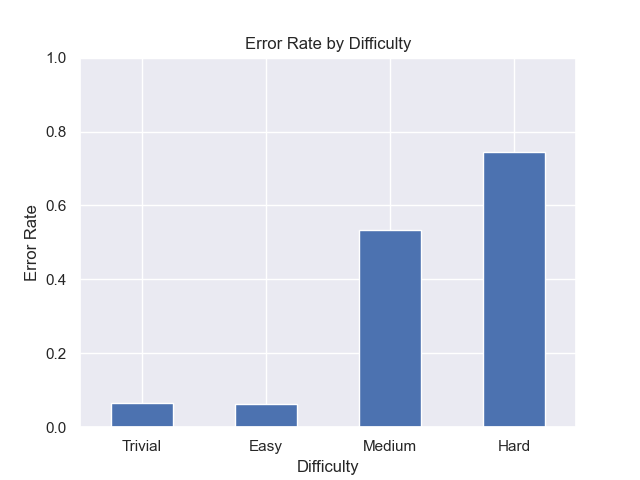
\includegraphics[width=0.5\textwidth]{figures/Data/Error_Rate_by_Difficulty.png}
  \caption[Error Rate by Difficulty]{The rate that errors occur for any given difficulty. }
  \label{fig:statistics_err_diff}
\end{figure}

\begin{figure}
  \centering
  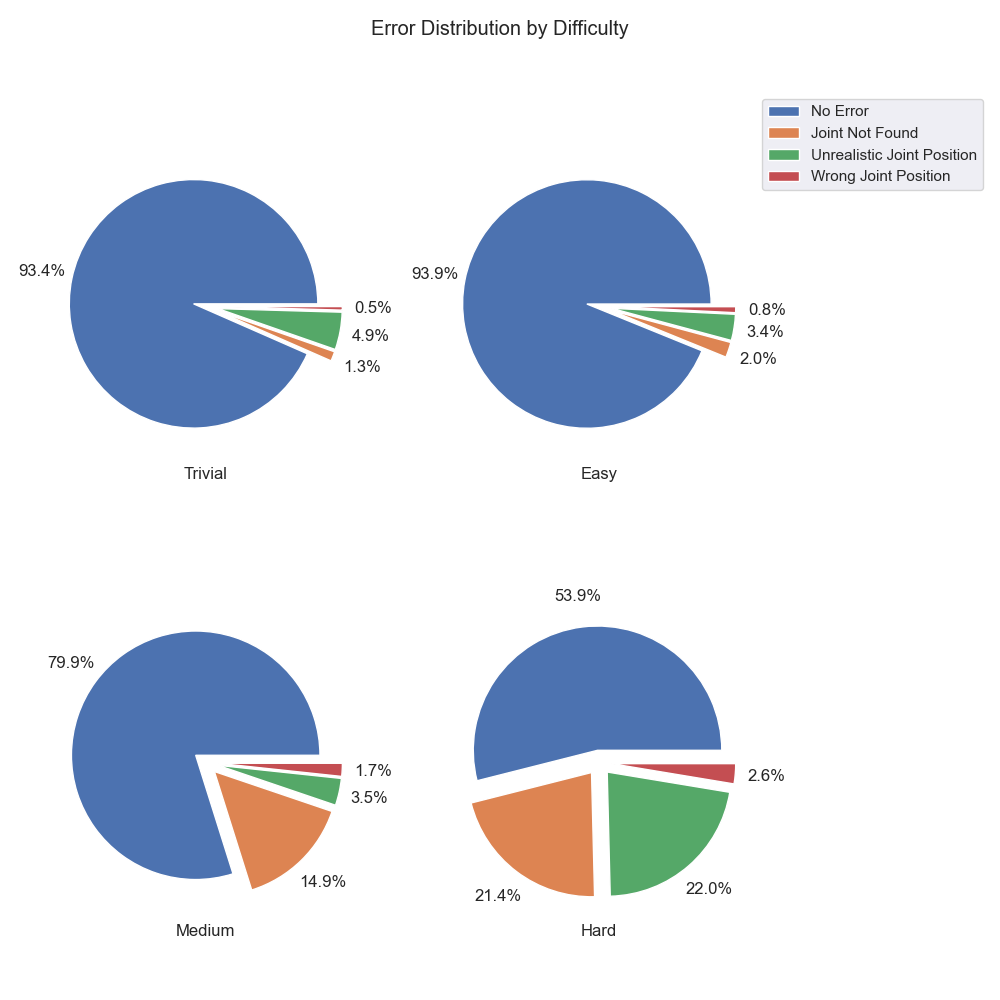
\includegraphics[width=0.5\textwidth]{figures/Data/Error_Distribution_by_Difficulty.png}
  \caption[Error Distribution by Difficulty]{The distribution of errors by difficulty. TODO}
  \label{fig:statistics_err_dist_diff}
\end{figure}

Some joints are more likely than others to be faulty, based on frequent occlusion, or generally more challenging detection. For example, hands and ankles are quite challenging to detect since they move frequently and are frequently occluded. On the other hand the head and the neck are least likely to be faulty. This distribution can be seen in Figure \ref{fig:statistics_err_dist_joint}, where the distribution of errors are shown for each joint. The joints are sorted by general occourence of errors.

\begin{figure}
  \centering
  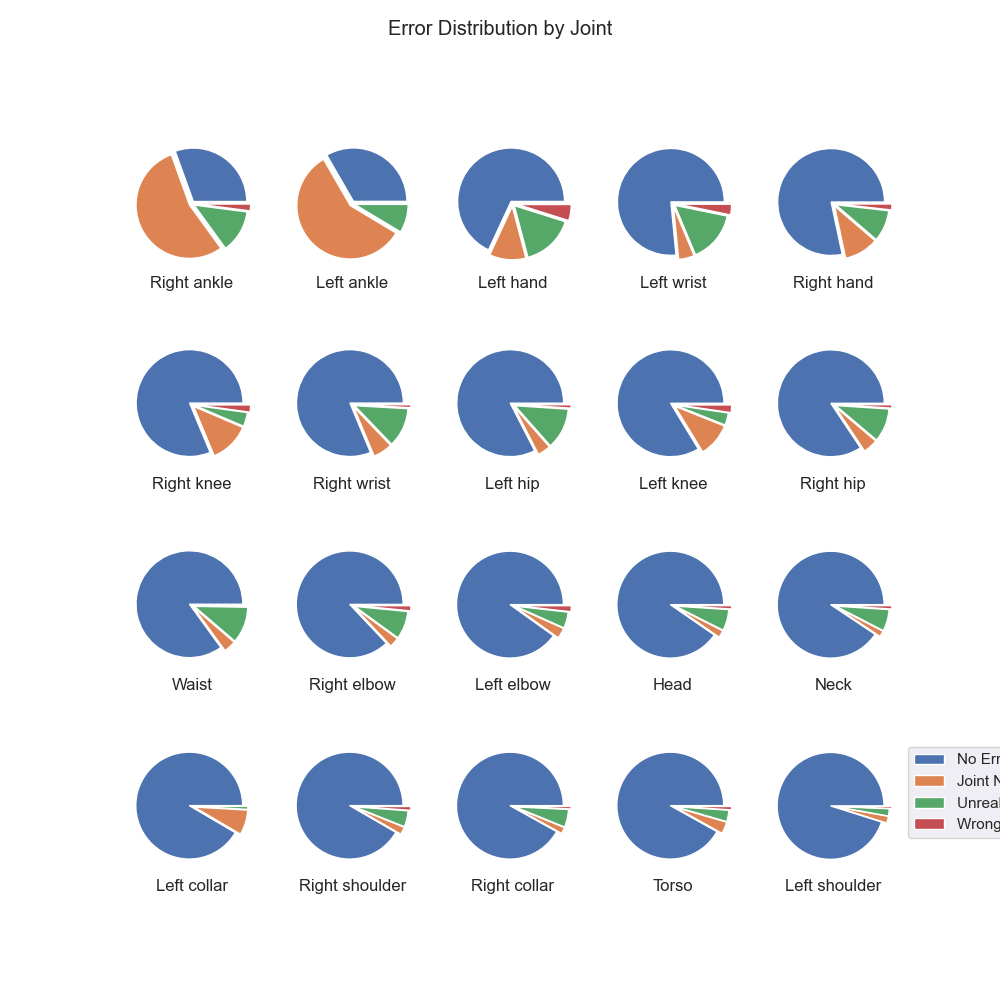
\includegraphics[width=0.5\textwidth]{figures/Data/Error_Distribution_by_Joint.png}
  \caption[Error Distribution by Joint]{The distribution of errors by Joint. TODO}
  \label{fig:statistics_err_dist_joint}
\end{figure}

\subsection{Problem Sets}
\label{sec:problem_set}